\documentclass[../../main.tex]{subfiles}
\begin{document}

\subsection*{7.6}
Una regione di spazio è sede di un campo elettrico $E = -E_{\vec{u_z}}$ con $E = 10^5\ \frac{V}{m}$ e di un campo magnetico $B = B_{\vec{u_z}}$ con $B=0.1\ T$.
\\Un protone viene immesso nella regione con $v_0 = 5 * 10^6\ \frac{m}{s}$ formante un angolo $\theta = 30°$ con l'asse z.
\\Mostrare che il protone percorre un'orbita elicoidale il cui asse è parallelo all'asse z.
\\a) Calcolare il raggio r dell'elica e la distanza $z_1$ percorsa dal protone nel primo giro.
\\b) Calcolare inoltre la distanza $z_0$ percorsa prima che il protone inverta il suo moto lungo z.
\\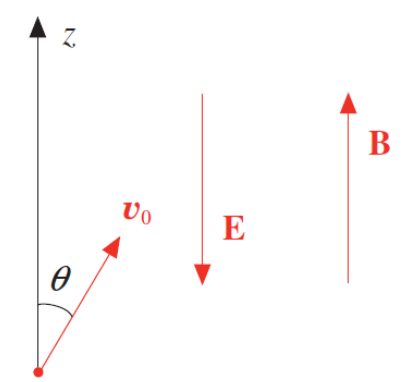
\includegraphics[scale=0.3]{e_7_6.png}
\subsubsection*{Formule utilizzate}
\subsubsection*{Soluzione punto a}
$v_{0z} = v_0\sin\theta$
\\$v_{0y} = v_0\cos\theta$
\\$\vec{F_L}= \left(q\ \vec{v_{0y}}\wedge\vec{B}\right)\vec{u_x}$
\\Utilizziamo solo la componente y di v perchè z è parallela.
\\ma $v_0z$ non è costante perchè c'è un campo che la modifica, E.
\\v cala con $\vec{F} = q\vec{E} = -ma$
\\$m_{az} = -qE$   $a_z = -\frac{qE}{m}$
\\$\vec{v_z} = \vec{v_0}t + \vec{a_z}t = \vec{v_0}t-\frac{q\vec{E}}{m}t$
\\$z = z_0 + v_0t + \frac{1}{2}at^2 = z_0 + \vec{v_0}t - \frac{q\vec{E}t}{m}-\frac{qEt^2}{2}$
\\$z_1 = z$ dopo 1 giro
\\T periodo di rotazione
\\$z_y = v_0\cos\theta T - \frac{1}{2}\frac{q}{m}ET^2$
\\$T = \frac{2\pi}{\omega}$ con $\omega = \frac{v_0\sin\theta}{r}$
\\Sia z* lo spazio percorso di fermarsi.
\\Dall'equazione del moto unformemente accellerato
\\$v_f^2 = v_i^2 + 2as$   $v_f = 0$
\\$v_i = v_0\cos\theta$   $a = -\frac{qE}{m}$   $s=z*$
\\abbiamo:
\\$(r_0\cos\theta)^2 = 2\frac{qE}{m}z*$
\\$z* = \frac{m_0v_o^2\cos^2\theta}{2qE}$
\subsubsection*{Soluzione punto b}
\newpage

\end{document}